

\chapter{Introduction}

%\label{chap:GettingStarted}
\section{Overview}
This section includes the overview of the report. 

\section{Motivation}

\subsection{Image Processing}






\section{Problem Statement}
This section includes problem statement

\section{Motivation}
Analyzing research interest and existing work in the field of IoT, security is the most vital issue that drives the researcher towards the field. As architecture and application is going large day by day, security has become the important challenge for IoT. Interest in this field is proportionally increases with the Heterogeneity of this network. 

\begin{figure}
    \centering
    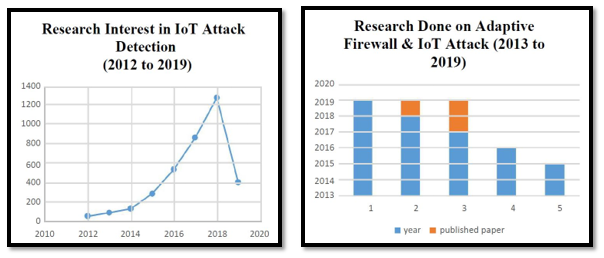
\includegraphics[scale=0.5]{Chap1/motivation.PNG}
    \caption{Research Interest in Field of IoT}
    \label{fig:motivation}
\end{figure}

 In figure \ref{fig:motivation} shows the existing research interest in IoT Attack Detection which is increasing day by day for last few years whereas for detecting attack concept of Adaptive Firewall is not so common and used term in this field. This drives us motivated to design adaptive firewall for attack detection and to block illegitimate traffic on IoT Network Model.
\section{Objective}
%The Overview goes here \cite{r1}.
IoT network model and devices are vulnerable to different kind of attacks. These attacks may vary to different category, so have different approach to detect and block them. The goal of this research is to study and identify potential IoT security attacks, detect and mitigate them by using Adaptive firewall concept. Additionally, machine learning should be considered for classifying attacks and identifying attacks \cite{c4}.
Specific goals of this thesis that should be mentioned:

\begin{itemize}
    \item Analyze network traffic to detect the malicious ones that tries to hamper the network.
    \item Find the characteristics of perception layer’s attack to identify specific attacks.
    \item Extract features from the generated traffic datasets to train machine learning classifiers and apply them to recognize attacks.Propose a centralized attack detection model.
    \item Design a rule based and ANN based FIS to help SDN controller to evaluate specific attack probability and block the suspicious ones.
    \item Maintaining the performance of the network.
\end{itemize}

This proposed model also answers the following questions:
\begin{enumerate}
    \item What are the major challenges that have guided security in IoT?
    \item What is the best attack detection way for IoT network model?
    \item Is there any generalized approach for detecting different layer attack?
    \item What is the best way to detect a single layer attack?
\end{enumerate}

\section{Assumptions \& Limitations}
Though a centralized and efficient model has been proposed to detect attacks on IoT network, it has limitations on which further studies should be done:
\begin{itemize}
    \item No approach has been mentioned for network and application layer security.
    \item No real time data has been used for the traffic analysis.
    \item Here feature Extraction and Selection method has been analyzed but no implementation has been shown.
    \item No comparison among different IDS model has been analyzed so can’t be declared it as the optimal way. 
    \item No performance measure of used Classifier is evaluated here.
\end{itemize}

\section{Research Outline}
Rest of the report is structured as follows: In \textbf{Chapter \ref{chap:2}} a literature study on related work is given including explanations for the most important terms used in this thesis-basic concept and architecture of IoT Network Model, Attacks on IoT, Concept and architecture of SDN, different model of IDS, Concept of Firewall has been discussed through this chapter. \textbf{Chapter III}  introduces system model including system architecture, algorithm and flowchart of working procedure of entire system model. \textbf{Chapter IV} explains the details of traffic analysis techniques, Feature Extraction and Selection mechanism and tools for this mechanism and reasoning how these mechanisms work for our model. \textbf{Chapter V} discusses about the simulation and model performance, to analysis result of the model it describes the basic mechanism of attack detection like Fuzzification, NSL KDD dataset, FIS, Defuzzification,Simulation and confusion matrix. Lastly in \textbf{Chapter VI} future work and conclusion is mentioned. 

\section{Limitation}
Bla bla bla
\label{sec:EffSearch} 
\index{Search engines!using effectively} %index will be created
%The rest of this report is organized as follows.

